\documentclass[tikz,border=4pt]{standalone}
% Shared look for the per-pattern diagrams. Copied from the IATEFL LTSIG talk
% (talks/doubly-personalised-language-learning/figures/llm-patterns.tex).
\usepackage{amssymb}
\usepackage{fontspec}
\setmainfont{Helvetica Neue}
\usetikzlibrary{arrows.meta,positioning,calc,fit}
\definecolor{ink}{HTML}{23373B}
\definecolor{hlc}{HTML}{C2410C}
\definecolor{okc}{HTML}{2E7D32}
\definecolor{badc}{HTML}{B91C1C}
\tikzset{
  mini/.style={rounded corners=2pt, minimum height=7mm, align=center,
               font=\small\color{ink}, fill=white, draw=ink!70, line width=0.6pt, inner sep=3pt},
  minillm/.style={mini, fill=hlc, draw=hlc, font=\small\bfseries\color{white}},
  fixed/.style={mini, fill=ink!12},                 % the fixed part of a prompt
  sarr/.style={-{Stealth[length=2mm]}, ink, line width=0.8pt},
  lbl/.style={font=\footnotesize\itshape\color{ink!75}},
  ok/.style={font=\small\bfseries\color{okc}},
  bad/.style={font=\small\bfseries\color{badc}},
}

\usetikzlibrary{backgrounds}
% Defensive Output Parsing: a provider that enforces a schema sends JSON straight
% to the check; one that does not needs its syntax repaired in code first. Either
% way code checks what no schema guarantees (complete, not refused, indices in
% range), and degrades to a fallback instead of raising.
\begin{document}
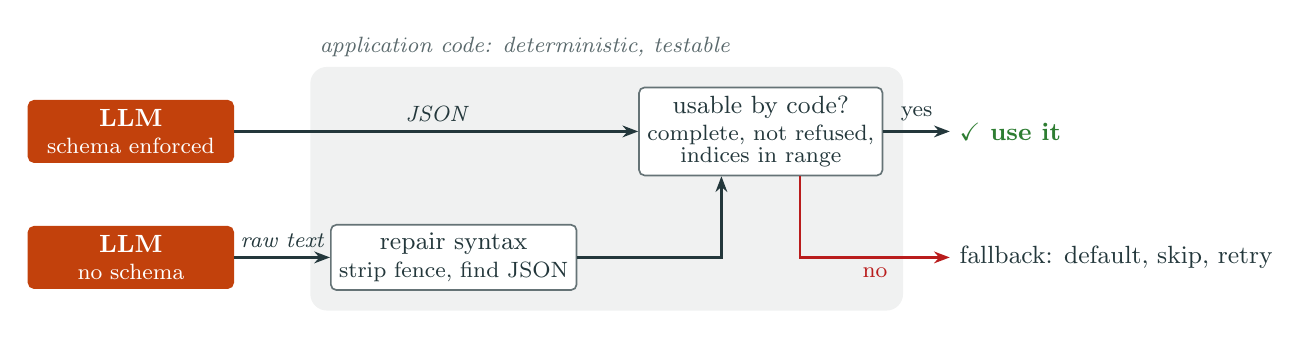
\begin{tikzpicture}[two/.style={align=center, font=\small\bfseries\color{white}}]
\node[minillm, minimum width=26mm, two] (l1) at (0,0) {LLM\\[-1pt]{\footnotesize\mdseries schema enforced}};
\node[minillm, minimum width=26mm, two] (l2) at (0,-1.6) {LLM\\[-1pt]{\footnotesize\mdseries no schema}};

\node[mini, minimum width=30mm, align=center] (fix) at (4.1,-1.6) {repair syntax\\[-1pt]{\footnotesize strip fence, find JSON}};
\node[mini, minimum width=30mm, align=center] (chk) at (8.0,0) {usable by code?\\[-1pt]{\footnotesize complete, not refused,}\\[-3pt]{\footnotesize indices in range}};
\draw[sarr] (l1) -- node[above, lbl] {JSON} (chk);
\draw[sarr] (l2) -- node[above, lbl] {raw text} (fix);
\draw[sarr] (fix.east) -| ([xshift=-5mm]chk.south);

\node[ok, anchor=west] (use) at (10.4,0) {\checkmark\ use it};
\draw[sarr] (chk) -- node[above, font=\footnotesize\color{okc}] {yes} (use);
\draw[sarr, color=badc] ([xshift=5mm]chk.south) |- node[pos=0.75, below, font=\footnotesize\color{badc}] {no} (10.4,-1.6);
\node[anchor=west, font=\small\color{ink}] at (10.4,-1.6) {fallback: default, skip, retry};

\begin{scope}[on background layer]
\node[fill=ink!7, rounded corners=6pt, inner sep=2.5mm, fit=(fix)(chk)] (code) {};
\end{scope}
\node[lbl, anchor=south west] at (code.north west) {application code: deterministic, testable};
\end{tikzpicture}
\end{document}
